% This must be in the first 5 lines to tell arXiv to use pdfLaTeX, which is strongly recommended.
\pdfoutput=1
% In particular, the hyperref package requires pdfLaTeX in order to break URLs across lines.

\documentclass[11pt]{article}

% Remove the "review" option to generate the final version.
\usepackage[review]{ACL2023}

% Standard package includes
\usepackage{times}
\usepackage{latexsym}

% For proper rendering and hyphenation of words containing Latin characters (including in bib files)
\usepackage[T1]{fontenc}
% For Vietnamese characters
% \usepackage[T5]{fontenc}
% See https://www.latex-project.org/help/documentation/encguide.pdf for other character sets

% This assumes your files are encoded as UTF8
\usepackage[utf8]{inputenc}

% This is not strictly necessary, and may be commented out.
% However, it will improve the layout of the manuscript,
% and will typically save some space.
\usepackage{microtype}

% This is also not strictly necessary, and may be commented out.
% However, it will improve the aesthetics of text in
% the typewriter font.
\usepackage{inconsolata}
\usepackage{listings}
\usepackage{graphicx}
% If the title and author information does not fit in the area allocated, uncomment the following
%
%\setlength\titlebox{<dim>}
%
% and set <dim> to something 5cm or larger.

\title{INFO 555 - Applied NLP Project 2}

% Author information can be set in various styles:
% For several authors from the same institution:
% \author{Author 1 \and ... \and Author n \\
%         Address line \\ ... \\ Address line}
% if the names do not fit well on one line use
%         Author 1 \\ {\bf Author 2} \\ ... \\ {\bf Author n} \\
% For authors from different institutions:
% \author{Author 1 \\ Address line \\  ... \\ Address line
%         \And  ... \And
%         Author n \\ Address line \\ ... \\ Address line}
% To start a seperate ``row'' of authors use \AND, as in
% \author{Author 1 \\ Address line \\  ... \\ Address line
%         \AND
%         Author 2 \\ Address line \\ ... \\ Address line \And
%         Author 3 \\ Address line \\ ... \\ Address line}

\author{Kiwoon Hong \\
  iSchool / Address line 1 \\
  Affiliation / Address line 2 \\
  Affiliation / Address line 3 \\
  \texttt{Kiwoon2799@arizona.edu} \\\And
  Second Author \\
  Affiliation / Address line 1 \\
  Affiliation / Address line 2 \\
  Affiliation / Address line 3 \\
  \texttt{email@domain} \\}

\begin{document}
\maketitle


\section{Introduction}

Detecting hate speech on social media platforms is critical to maintaining a safe and inclusive online environment. Hate speech not only fosters discrimination and harm, but also leads to an imbalance in digital discourse by silencing the voices of certain groups. As social media has had a huge impact in modern society, hateful content can have far-reaching consequences, including social division and mental health impacts. Therefore, implementing effective hate speech detection is essential to encourage respectful interactions, protect communities, and ensure that social media remains a healthy platform.\\
This project aims to annotate hate speech by sampling tweets. However, detecting hate speech is a challenging task due to its complex and sensitive nature. Hate speech can take many forms, from obvious blames to subtle slang that only certain groups recognize. Cultural, linguistic, political, and regional differences also complicate the identification process, as what one group feels is hate speech may not be to another. This complexity often leads to problems with automated systems and human annotation, such as over-censorship or failure to detect offensive content. \\
Tweets Hate Speech Detection dataset\footnote{\url{https://huggingface.co/datasets/tweets-hate-speech-detection/tweets_hate_speech_detection}} on Hugging Face contains a variety of tweets, including about 7 percent labeled hate speech, and 93 percent labeled non-hate speech.


\section{Related Work}

Hate speech annotation is an active area of research. In particular, the problem of hate speech ambiguity mentioned in the introduction has also been addressed. paper by \citet{assimakopoulos-etal-2020-annotating}, acknowledged this ambiguity and used 10 years of online commentary data and focused on context and hidden messages using Critical Discourse Analysis(CDA). As a result, they suggested that a multi-layer annotation scheme rather than a dichotomous distinction might be useful. \citet{ron-etal-2023-factoring} decomposed the expressions into multidimensional factors. After filtering and sampling tweets about Jews, we decomposed the hateful expressions into five categories for annotation. \\ However, these two prior studies were characterized by a multilayered categorization of hate speech about specific groups. Therefore, it is difficult to generalize the classification of general tweets into specific groups and subcategories according to their respective distinction principles. 

\section{Procedure}
\subsection{Experiment}
\subsubsection{Data}
This \texttt{tweets\_hate\_speech\_detection} dataset is extracted from the Hugging Face dataset provided by Roshan Sharma, which is divided into a training set of 31,962 data and a test set of 17,197 data. The training set consists of English tweets from Twitter users and their hate speech labels (1 for hate speech, 0 for not hate speech), while the test set consists of tweets only. The distribution of labels in the train data is biased. Only 2,242 data points, about 7\% of the data, are labeled as hate speech. Therefore, given that this may cause difficulties in annotation, the data was first undersampled to match the number of hate speech, and then resampled 300 random tweets. After checking the label distribution, the labels were removed for annotation, leaving only the tweet text for annotation.
\subsubsection{Annotation Protocol}
The project has a total of two annotators, with the annotator tagging the data themselves and one additional LLM acting as a reference. The first annotator is the researcher. He is a master's student in data science, does not use Twitter, is not a native English speaker, and is not an American citizen, so he does not have expertise in American culture. The second annotator is Noah (an alias). He is an undergraduate physics student, has been on Twitter, is a native English speaker, and is a U.S. citizen. Both annotators shared the same guidelines for hate speech The data annotation was based on the definition of hate speech provided by the UN's \texttt{What is hate speech}\footnote{\url{https://www.un.org/en/hate-speech/understanding-hate-speech/what-is-hate-speech}} article. Only two labels were allowed: \texttt{'hate'} and \texttt{'nohate'}.\\
The LLM model used as a comparison group for data annotation is the HuggingFace's 
\texttt{roberta-hate-speech-dynabench-r4-target}\footnote{\url{https://huggingface.co/facebook/roberta-hate-speech-dynabench-r4-target}} model. This model is from a paper by \citet{DBLP:journals/corr/abs-2012-15761}, proposing a method for building dynamically trainable datasets and develops a model that can effectively handle new types of expressions and covert hate in hate speech detection.

\subsection{Summary Statistics}
The 300 tweets were tagged by two annotators and an LLM model. The researcher tagged 55 hate speech, Noah tagged 37, and the LLM model tagged 37. This means that 18.33\%, 12.33\%, and 12.33\% of the total data was tagged as hate speech, respectively, which is significantly less than the previous 50\% of undersampling.

\subsection{Inter Annotator Agreement}
The quality of the data was verified using IAA between the two annotators and between the annotators and LLM. Cohen's kappa score was used. In addition, tweets with tagging mismatches between two annotators and tweets with mismatches between annotators and the model were extracted for further analysis.
\subsection{Demonstrating and Utilization}
A simple Logistic Regression baseline model was created using the annotations of the two annotators, and the accuracy and the F1 score of the models were measured. Since there were no labels for the test part of this dataset, the test set was sampled by performing a sampling without replacement on the train part.

\section{Results}
The statistics and figures are attached in the appendix.
\subsection{IAA}
The Cohen's kappa score between the two annotators is 0.59, showing weak to moderate agreement. On the other hand, the researcher and LLM have a weak agreement of 0.46 and Noah and LLM have a weak agreement of 0.44.
\subsection{Logistic Regression}
Both models based on the data from the two annotators predicted the test data as 'nohate', resulting in low performance.
\subsection{Error Analysis}
Compared to Noah, the investigator was better able to identify non-American ethnicity discrimination and tag it as hate. For example:
\begin{verbatim}
#koreans &amp; joseon people in japan,
will abuse the  for claims of own 
rights by rough demo.  #aberdeen
\end{verbatim}
In contrast, Noah was better at recognizing hate speech related to US politics:
\begin{verbatim}
#intrumpsamerica extending your hand &amp;
uniting merica is unprecedented!
#rapist #egomaniac @user
\end{verbatim}
\section{Conclusion}
Common hate speech had moderate matches. However, due to the the subcultural nature of social media and different sensitivities to specific category of hate speech even though they got the same guidelines, overall, the agreement was weak. Therefore, as mentioned in the related work above, detecting hate speech is a very nuanced task, and it is important to recruit annotators with diverse knowledge, cultures, environments, and memes.
\subsection{Limitations}
The dataset contained a large number of emojis, which had conversion issues due to Unicode and thus could not be fully interpreted. Also, both annotators could not understand tweets about cultures they did not belong to. Finally, a more appropriate demonstration model needs to be chosen based on less data rather than a Logistic Regression model.
% Entries for the entire Anthology, followed by custom entries
\bibliography{anthology,custom}
\bibliographystyle{acl_natbib}
\appendix

\section{Appendix}
\label{sec:appendix}


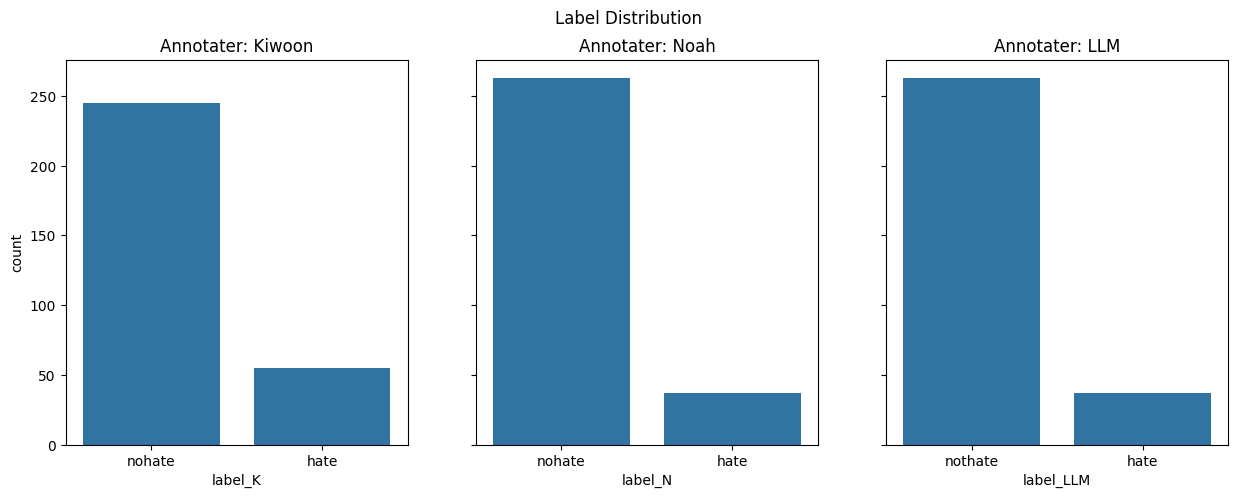
\includegraphics[width=16cm]{figure/figure1.png}
\\

\begin{table}[ht]
\centering
\begin{tabular}{lll}
\hline
\textbf{Model} & \textbf{Accuracy} & \textbf{F1 score} \\ 
\hline
Model\_Kiwoon& 55\% & 0.688 \\ 
Model\_Noah& 52\% & 0.684 \\ 
\end{tabular}
\caption{\label{citation-guide}
Accuracy \& F1 Score for each model based on two annotators.
}
\end{table}

\end{document}
